% ******************************************************** %
%              TEMPLATE DE INFORME ORGA2 v0.1              %
% ******************************************************** %
% ******************************************************** %
%                                                          %
% ALGUNOS PAQUETES REQUERIDOS (EN UBUNTU):                 %
% ========================================
%                                                          %
% texlive-latex-base                                       %
% texlive-latex-recommended                                %
% texlive-fonts-recommended                                %
% texlive-latex-extra?                                     %
% texlive-lang-spanish (en ubuntu 13.10)                   %
% ******************************************************** %


\documentclass[a4paper]{article}
\usepackage[spanish]{babel}
\usepackage[utf8]{inputenc}
\usepackage{charter}   % tipografia
\usepackage{graphicx}
%\usepackage{makeidx}
\usepackage{paralist} %itemize inline

%\usepackage{float}
%\usepackage{amsmath, amsthm, amssymb}
%\usepackage{amsfonts}
%\usepackage{sectsty}
%\usepackage{charter}
%\usepackage{wrapfig}
%\usepackage{listings}
%\lstset{language=C}

% \setcounter{secnumdepth}{2}
\usepackage{underscore}
\usepackage{caratula}
\usepackage{url}


% ********************************************************* %
% ~~~~~~~~              Code snippets             ~~~~~~~~~ %
% ********************************************************* %

\usepackage{color} % para snipets de codigo coloreados
\usepackage{fancybox}  % para el sbox de los snipets de codigo

\definecolor{litegrey}{gray}{0.94}

\newenvironment{codesnippet}{%
	\begin{Sbox}\begin{minipage}{\textwidth}\sffamily\small}%
	{\end{minipage}\end{Sbox}%
		\begin{center}%
		\vspace{-0.4cm}\colorbox{litegrey}{\TheSbox}\end{center}\vspace{0.3cm}}



% ********************************************************* %
% ~~~~~~~~         Formato de las páginas         ~~~~~~~~~ %
% ********************************************************* %

\usepackage{fancyhdr}
\pagestyle{fancy}

%\renewcommand{\chaptermark}[1]{\markboth{#1}{}}
\renewcommand{\sectionmark}[1]{\markright{\thesection\ - #1}}

\fancyhf{}

\fancyhead[LO]{Sección \rightmark} % \thesection\ 
\fancyfoot[LO]{\small{Nombre Apellido, Nombre Apellido, Nombre Apellido}}
\fancyfoot[RO]{\thepage}
\renewcommand{\headrulewidth}{0.5pt}
\renewcommand{\footrulewidth}{0.5pt}
\setlength{\hoffset}{-0.8in}
\setlength{\textwidth}{16cm}
%\setlength{\hoffset}{-1.1cm}
%\setlength{\textwidth}{16cm}
\setlength{\headsep}{0.5cm}
\setlength{\textheight}{25cm}
\setlength{\voffset}{-0.7in}
\setlength{\headwidth}{\textwidth}
\setlength{\headheight}{13.1pt}

\renewcommand{\baselinestretch}{1.1}  % line spacing

% ******************************************************** %


\begin{document}


\thispagestyle{empty}
\materia{Organización del Computador II}
\submateria{Segundo Cuatrimestre de 2014}
\titulo{Trabajo Práctico II}
\subtitulo{subtitulo del trabajo}
\integrante{Nombre}{XXX/XX}{mail}
\integrante{Nombre}{XXX/XX}{mail}

\maketitle
\newpage

\thispagestyle{empty}
\vfill
\begin{abstract}
En el presente trabajo se describe la problemática de ...
\end{abstract}

\thispagestyle{empty}
\vspace{3cm}
\tableofcontents
\newpage


%\normalsize
\newpage

\section{Objetivos generales}

El objetivo de este Trabajo Práctico es comparar el rendimiento entre implementación en C y ASM
usando el set de instrucciones SSE (en un entorno donde es posible usar programación vectorial).


\section{Contexto}

\begin{figure}
  \begin{center}
	
\includegraphics[scale=0.66]{img/logouba.jpg}
	\caption{Descripcion de la figura}
	\label{nombreparareferenciar}
  \end{center}
\end{figure}


\paragraph{\textbf{Titulo del parrafo} } Bla bla bla bla.
Esto se muestra en la figura~\ref{nombreparareferenciar}.



\begin{codesnippet}
\begin{verbatim}

struct Pepe {

    ...

};

\end{verbatim}
\end{codesnippet}


\section{introduccion} 
Este trabajo practico consiste en implementar filtros gráficos utilizando el modelo de procesamiento SIMD. 
El mismo consta en dos componentes igualmente importantes. En primer lugar aplicaremos lo estudiado en clase programando de manera vectorizada un conjunto de filtros.\\
Se realizarán 4 filtros:\\
\begin{itemize}
    \item Tres Colores
    \item Efecto Bayer
    \item Cambia Color
    \item Edge Sobel
\end{itemize}
El filtro Tres Colores es usado para ...\\
El filtro Bayer es usado para ... . La razón de que se use mayor cantidad de puntos verdes es que el ojo humano es más sencible a ese color.\\
EL filtro Cambia Colores es usado para ...\\
El cuarto filtro es Edge Sobel, el cual utiliza la vecindad de Moore para hacer una aproximaci\'on de las derivadas parciles, este filtro es \'util para poder detectar los bordes de la imagen.\\


\section{desarrollo} 

Se compararán los filtros implementadas en lenguage C compilada con máximas optimizaciones (o3) y la versión ASM utilizando el set de instrucciones
SSE. \\
Para medir el rendimiento usaremos la cantidad de ciclos de ejecución, en particular se tomara la mediana de las mediciones.\\
Se útilizara el registro Time Stamp Counter(TSC) que es global del procesador y se ve afectado por una serie de factores,
como por ejemplo el scheluder para realizar un cambio de contexto, esto implicará contar muchos más ciclos (outliers)
 que si nuestra función se ejecutara sin interrupciones, con lo cual se decide tomar la mediana que es robusta a outliers.\\
El procesamiento digital de imágenes es el conjunto de técnicas que se aplican a las imágenes digitales con el objetivo de mejorar la calidad o facilitar la búsqueda de información. 
\\
Siempre se hacen las cuentas independientemente del contenido de la imagen en si.\\

\subsubsection{edgeSobel}
El algoritmo comenzara llenando la parte que se procesa (toda la matriz, excepto los bordes),
y luego completara los bordes de la matriz con 0.\\
Tiene cuatro diferentes tipos de iteraciones y un caso que es tratado de forma diferente.\\
\textbf{caso 1}:\\
	Llenado de la matriz con los pixeles procesados, se excluyen los bordes pues no se pueden aplicar los operadores.\\
\textbf{caso 2}:\\
	Llenado de la última fila a procesar.\\
\textbf{caso 3}:\\
	Llenado de los bordes de los costados.\\
\textbf{caso 4}:\\
	El ultimo caso es para poder llenar la primer fila y la ultima con ceros, la forma de iterar es la misma pero cambia el lugar desde donde inicia cada una.\\

\textbf{1. Llenado de los pixeles procesados usando parte baja de un xmm}:\\ Se tomara la parte baja de un registro xmm y los 8 bytes de la parte baja serán extendidos a 8 words para que al hacer las cuentas no perdamos precisión, como se calcularán 4 pixeles, estaremos trabajando con 6 bytes, los 10 bytes restantes no se utilizarán. Esto solo sirve para llenar parte de la matriz, por que al querer seguir iterando, llegaremos a la última posición y necesitariamos leer 10 bytes demás, pero nos saldriamos de la matriz.\\

\textbf{2. Llenado de los pixeles procesadosusando parte alta de un xmm}:\\ Responde al problema que surgio anteriormente, entonces ahora al leer en un registro xmm tranjaremos con la parte alta, como necesitamos procesar 4 pixeles a la hora de acceder a la matriz necesitaremos estar 10 bytes (posiciones) atras, asi poder acceder a los 6 bytes con los que se procesan 4, luego por la forma en como iniciamos y dado que la cantidad de pixeles en la fila es muliplo de 8, no podremos  procesar los dos ultimos bytes y estos se harán como caso aparte.\\

\textbf{3. Llenado de los bordes de los costados}:\\ La matriz es accedienda desde último byte de la primer fila, copia su valor en un xmm, hace un shift de 2 bytes para poner los 2 primeros bytes en 0 y luego un shift de 2 bytes para reacomodar, con esto se puso en 0 los 2 byte de los costados, luego se incementa en cantidad de columnas a la posición y se procede de la misma forma hasta llegar a la ante-ultima fila.\\

\textbf{4. Llenado de los bordes superior e inferior}:\\
	Para la \textbf{primer fila}, primero se lee con el registro xmm y se shiftean 8 bytes, se divide la cantidad de columnas por 8 y se procede a iterar cantidad de (cantidad de pixeles en fila/8)-1 para poder llenas la primer fila.\\
	Para la \textbf{ultima fila}, se lee desde 8 bytes antes y se hace un shift para poder poner en 0 los primeros 8 bytes de la ultima fila, luego se procede a iterar cantidad de (cantidad de pixeles en fila/8)-1 para poder llenar la matriz.\\


\subsubsection{Tres Colores}
Este filtro tiene una sola forma de iterar, y en cada itecarión procesa 4 pixeles. Primero extiende a dword cada componenete, para que al hacer la suma no exceda, luego hace una conversión a float y divide por 3 obteniendo W, luego procesa los colores crema, verde y rojo para cada pixel.\\
\textbf{Descripción de una iteración}:\\
Leer de memoria:\\
$Xmm0 = [argb| argb| argb | argb].$\\
Se hacen 3 copias y se las shiftean para tener cada componente en dword:\\ 
$Xmm1 = [r| r| r| r]$\\
$Xmm2 = [g| g| g| g]$\\
$Xmm3 = [b| b| b| b]$\\
Se obtiene la suma en dword:\\
$Xmm1 = [r+g+b| r+g+b| r+g+b| r+g+b]$\\
Se castean a float single precisión, se divide por 3 y se castea a int:\\
$Xmm1 = [0,0,0,W| 0,0,0,W| 0,0,0,W| 0,0,0,W]$(estan en dword, pero ocupan 1 byte)\\
Se acomoda $Xmm1$ para que tenga los 3 bytes de cada dword cargado con $W$:\\
$Xmm1 = [0,W,W,W| 0,W,W,W| 0,W,W,W| 0,W,W,W]$\\
Se acomoda en $Xmm2$ los $W$ de los dos primeros píxeles y en $Xmm3$ los $W$ de los dos segundos píxeles:\\
$Xmm2 = [0,0,0,W|0,W,0,W|0,W,0,W|0,W,0,W]$\\
$Xmm3 = [0,0,0,W|0,W,0,W|0,W,0,W|0,W,0,W]$\\
Se limpa $Xmm0$ para que sea acumulador:\\
$Xmm0 = [0|0|0|0]$\\
Se procesan los crema y con un pand se filtra los que dieron negativo:\\
$Xmm0 = [cremas|cremas|cremas|cremas]$\\
Se procesan los verdes y con un pand se filtra los que dieron negativo:\\
$Xmm0 = [cremas y verdes|cremas y verdes|cremas y verdes|cremas y verdes]$\\
Se procesan los rojos y con un pand se filtra los que dieron negativo:\\
$Xmm0 = [rojos, cremas y verdes|rojos, cremas y verdes|rojos, cremas y verdes|rojos, cremas y verdes]$\\
Se escribe a memoria.\\
\subsubsection{Efecto Bayer}

\subsubsection{Cambia Color}

\section{Experimentación}
En la siguiente experimentación realizaremos comparaciones entre el código escrito en ASM contra el escrito en C++ con optimización nivel 3.

Para medir el rendimiento usaremos la cantidad de ciclos de ejecución, en particular se tomara la mediana de las mediciones.

Se útilizara el registro Time Stamp Counter (TSC) que es global del procesador y se ve afectado por una serie de factores, como por ejemplo el scheluder para realizar un cambio de contexto, esto implicará contar muchos más ciclos (outliers) que si nuestra función se ejecutara sin interrupciones, con lo cual se decidió tomar la mediana que es más robusta dadas las condiciones. En los experimentos contemplaremos el valor de un lado de la imagen, que interpretamos como matriz, en el eje X y en el eje Y tomaremos la mediana de la cantidad de clocks que toma dicha matriz con la función.



\subsection{Tres Colores}

El primer experimento comienza con la función de Tres Colores. Uno de las primeras aproximaciones de los resultados que estimamos fue una mejora

\vspace{6px}
\begin{center}
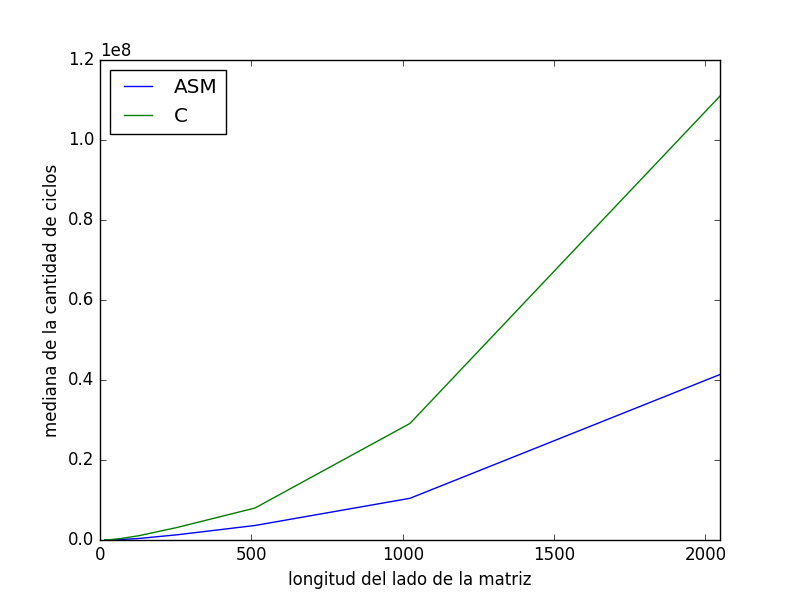
\includegraphics[width=12.5cm, height=9
cm]{images/car_tresColores.png}
\end{center}
\vspace{6px}


Como podemos observar la diferencia entre ASM y C es notoria. Esto se debe al paralelismo que se maneja en las instrucciones de SSE que se propuso utilizar en este trabajo. 

\subsection{Efecto Bayer}

La segunda experimentación que se realizó fue con el filtro de $Efecto$ $Bayer$, este mismo filtro deja solo uno de los 3 colores representantes de los píxeles con un patrón determinado. Como primera idea de las posibles mejoras que surgen a partir de utilizar ASM en vez de C, son los accesos a memoria. En general la cantidad de accesos a memoria se reduce, ya que trabajamos con múltiples píxeles al mismo tiempo. Este filtro no es la excepción y al traer de memoria 4 píxeles en vez de 1, como se haría con C, se mejoran mucho los tiempos. Continuemos con los resultados:


\vspace{6px}
\begin{center}
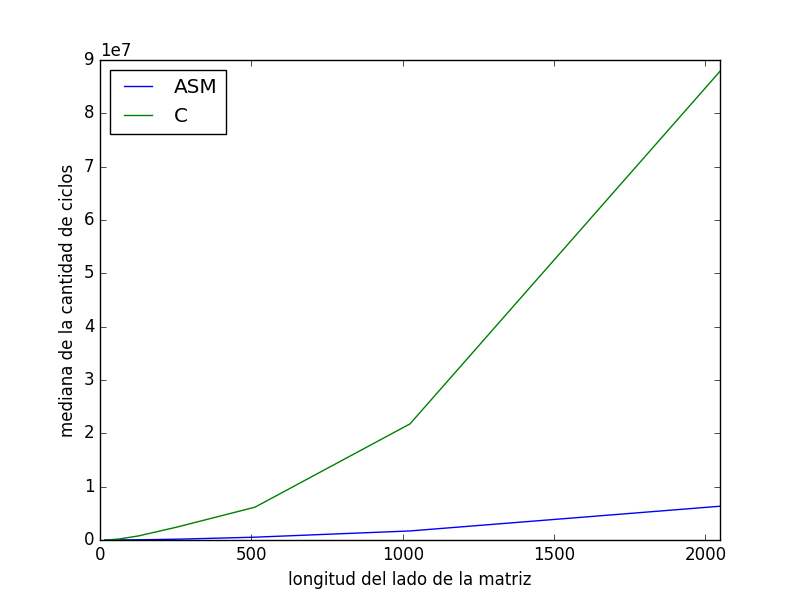
\includegraphics[width=12.5cm, height=9
cm]{images/car_efectoBayer.png}
\end{center}
\vspace{6px}

Podemos observar como el cambio es bastante alto con respecto a la implementación en C. Esto se debe, principalmente, a los accesos a memoria. Sin embargo, las operaciones que realizan las instrucciones de SSE influyen en los cambios de tiempo ya que se realizan simultáneamente.



\subsection{Edge Sobel}

La cantidad de operaciones que se realizan sobre en este filtro es bastante más que las que venimos trabajando anteriormente, por lo que uno de los posibles cambios en comparación con C, es que en ASM va a mejorar bastante el tiempo.


\vspace{6px}
\begin{center}
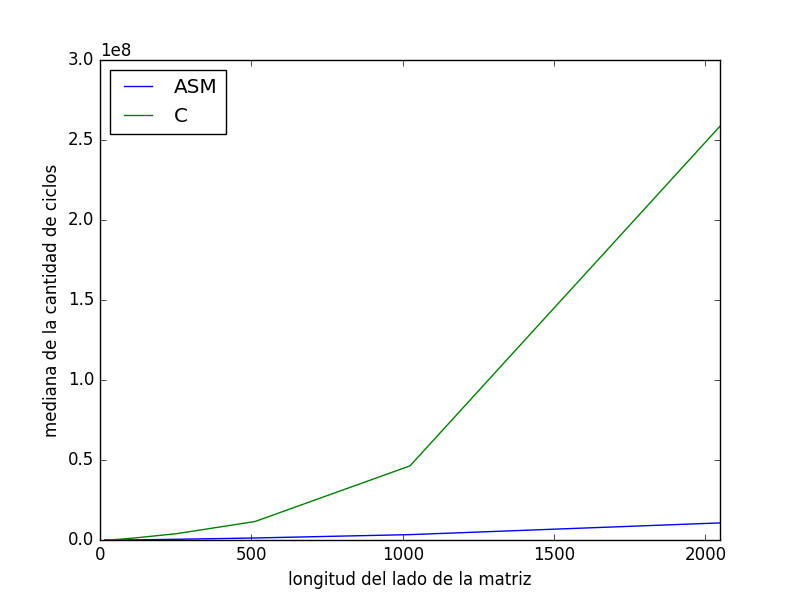
\includegraphics[width=12.5cm, height=9
cm]{images/car_edgeSobel.png}
\end{center}
\vspace{6px}





\subsection{Cambia Color}

En el caso de $Cambia$ $Color$ esperamos un cambio considerable ya que los accesos a memoria que se realizan dentro de cada iteración son 2, uno para traer los datos y otro para escribir. 

\vspace{6px}
\begin{center}
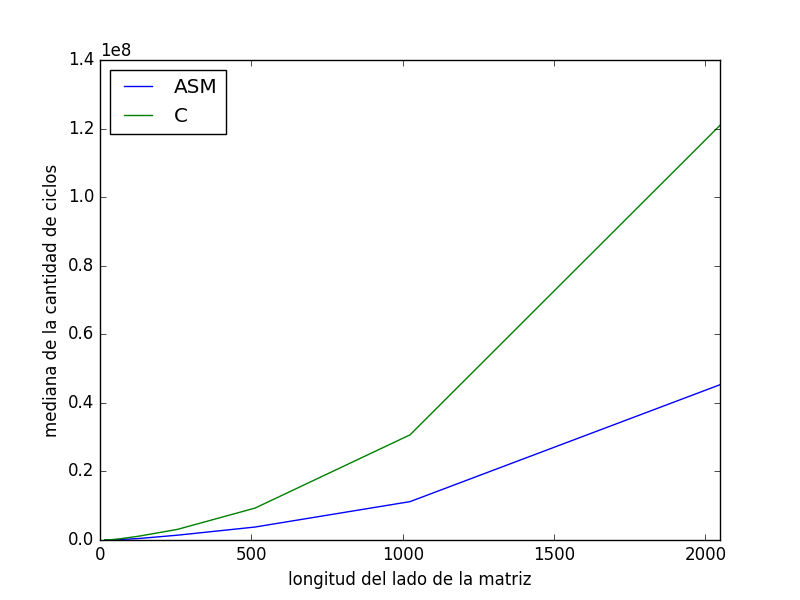
\includegraphics[width=12.5cm, height=9
cm]{images/car_cambiaColor.png}
\end{center}
\vspace{6px}

Podemos ver que el cambio es considerable, aunque no tanto como en otros filtros. Luego de un análisis se llegó a la conclusión de que el cambio de tiempos es bueno, aunque no mejor que otros filtros, debido a la cantidad de operaciones que tiene una iteración a comparación de los demás filtros. 

\section{Conclusiones y trabajo futuro}
Como conclusión general, podemos ver como los cambios en ASM y C se pronuncian en cada uno de los filtros. Así vemos como poder trabajar a más bajo nivel para situaciones específicas puede resultar muy beneficioso si lo que buscamos es optimizar los tiempos, como contraparte es más complejo trabajar en ASM que en C.


\subsection{Tres Colores y Efecto Bayer}

En estos dos filtros nos resulto importante destacar que los cambios de ASM a C fueron considerablemente distintos en los códigos de cada uno. En $Efecto$ $Bayer$ las mejoras fueron mucho más notables que en $Tres$ $Colores$, vale aclarar que esto es en comparación a C, no en tiempos concretos ya que el filtro $Efecto$ $Bayer$ tarda más en general que el segundo. 

Estamos convencidos que esta diferencia de mejoras se debe a la utilización de instrucciones como $Shuffle$ en $Tres$ $Colores$, que es una instrucción costosa. También existe una cantidad más grande de instrucciones que se utilizan para calcular el filtro de $Tres$ $Colores$



\end{document}

